%--------------------------
\subsection{Component}
%--------------------------

Formally in \mad, a component is defined as a tuple that can be divided
into four different parts: \emph{places}, \emph{transitions}, \emph{ports} and
\emph{bindings}.

\paragraph{Places}{

A component in \mad is first defined by a set of \emph{places} denoted
$\Pi$. A component is also defined by two sets of
\emph{docks}. A dock is represented by a small square and is attached to a
place. It is used to handle synchronization of parallel branches. The
first set concerns input docks. It is denoted $\Delta_{i}$ and it is
displayed under the place they are attached to. The second set is
denoted $\Delta_{o}$. It contains output docks and is displayed above
the place they are attached to.
The function $place\,:\,\Delta_{o}\cup\Delta_{i}\rightarrow\Pi$
returns the place a dock is attached to. Functions
$dock_i\,:\,\Pi\rightarrow \mathcal{P}(\Delta_{i})$ and
$dock_o\,:\,\Pi\rightarrow \mathcal{P}(\Delta_{o})$ respectively
returns the subset of $\Delta_i$ and $\Delta_o$ attached to a place
$\pi\in\Pi$. Places can be part of one or multiple groups which are
subsets of $\Pi$. The set of groups is denoted $G$. Last, $I \subseteq \Pi$ is the
non-empty set of initial places of the component.

}

\paragraph{Transitions}{

  % -----
\begin{table}[tp]
  \centering
  \resizebox{\columnwidth}{!}{%
    \begin{tabular}{|c|c|}
      \hline
      & \emph{Places}\\
      \hline
      $\Pi$ & set of places of a component\\
      $\Delta_{i}$ & set of input docks of a component\\
      $\Delta_{o}$ & set of output docks of a component\\
      $place$ & function mapping a dock to its place\\
      $dock_{i}$ & function mapping a place to its input docks\\
      $dock_{o}$ & function mapping a place to its output docks\\
      $G$ & set of groups of places\\
      $I$ & subset of places holding a token at initialization\\
      \hline
      \hline
      & \emph{Transitions}\\
      \hline
      $\Theta$ & finite set of transitions\\
      $A$ & finite set of actions\\
      $action$ & function mapping a transition to its corresponding action\\
      $end$ & function indicating if the action of the transition has finished\\
      \hline
      \hline
      & \emph{Ports}\\
      \hline
      $P_{u}$ & set of use ports of a component\\
      $P_{p}$ & set of provide ports\\
      $T_{port}$ & set of types of ports\\
      $type_{p}$ & function mapping a port to its type\\
      $D_{u}$ & set of data use ports of a component\\
      $D_{p}$ & set of data provide ports\\
      $T_{data}$ & set of types of data ports\\
      $type_{d}$ & function mapping a data port to its type\\
      $\mathbb{D}$ & set of possible data values\\
      \hline
      \hline
      & \emph{Bindings}\\
      \hline
      $B_{P_{u}}$ & set of pairs mapping use ports to transitions\\
      $B_{P_{p}}$ & set of pairs mapping provide ports to groups of places\\
      $B_{D_{u}}$ & set of pairs mapping data use ports to transitions\\
      $B_{D_{p}}$ & set of pairs mapping data provide ports to places\\
      \hline
      \hline
      & \emph{Assembly}\\
      \hline
      $C$ & set of component instances of an assembly\\
      $L_{P}$ & set of use-provide connections of an assembly\\
      $L_{D}$ & set of data-use-provide connections of an assembly\\
      $ebl$ & function indicating if a connection is enabled\\
      \hline
      \hline
      & \emph{Semantics}\\
      \hline
      $mk$ & function indicating if an element holds a token\\
      $val_{A,D_p}$ & returns the value given by an action to a data-provide port\\
      $val$ & function mapping a data provide port to its current value\\
      \hline
    \end{tabular}
  }
  \caption{Notations used throughout this paper}
  \label{tab:not}
\end{table}
%-----
A component is also defined by a set of \emph{transitions} denoted
$\Theta$. A transition $\theta \in \Theta$ is a pair containing one
source dock and one destination dock: $\theta =
\left(s,d\right)\,:\,s\in\Delta_{o},\,d\in\Delta_{i}$. 
%\CP{d=i $=>$ i is not defined! $d\in\Delta_i$ tout simplement, non ?}.
%
Each transition is associated to an \emph{action}. The set of actions is
denoted $A$ and the function $action\,:\,\Theta\rightarrow A$ gives the action
associated to a given transition. Finally, the function
$end\,:\,A\rightarrow\mathbb{B}$, where $\mathbb{B}=\left\{
\text{true},\text{false}\right\}$ indicates whether the action of a
transition has finished.
  
}

\paragraph{Ports}{

Places and transitions are internal elements of a \mad component.
The external interfaces of a component in \mad is
composed of \emph{ports}. A component contains a set of \emph{use-ports}
denoted $P_{u}$, and a set of \emph{provide-ports}, denoted
$P_{p}$. Each port is associated to a type in $T_{port}$, and the
function $type_{p}\,:\,P_{u}\cup P_{p}\rightarrow T_{port}$ maps the ports
to their type. 

In addition to traditional use-provide ports of component models,
\mad handles a specific use-provide abstraction for the
transfer of data values. These ports are called \emph{data-use-ports}
and \emph{data-provide-ports}. The set of data-use ports is denoted
$D_{u}$, and the set of data-provide ports is denoted
$D_{p}$. The set of possible data values is denoted
by $\mathbb{D}$. Finally, the function $type_{d}\,:\,D_{u}\cup
D_{p}\rightarrow T_{data}$ returns the data type of a given data port. In
  
}

\paragraph{Bindings}{

In a \mad component, places, groups of places and transitions can be
bound to ports through \emph{bindings}. There are four sets of bindings.
First, we denote $B_{P_{u}}$ the set of pairs that maps
each use port to one or multiple internal transitions in $\Theta$, indicating
that these transitions use the service associated to this port: 
$\left(p,\theta\right)\,:\,p\in P_{u},\,\theta\in\Theta$. Second, we
denote $B_{P_{p}}$ the set of pairs that maps each provide port to one or
multiple groups of places, indicating that if at least one token exists in each
group, the port is active: $\left(p,g\right)\,:\,p\in
P_{p},\,g\in G$. Third, we denote $B_{D_{u}}$ the set of pairs that
maps each data use port to one or multiple internal transitions in $\Theta$,
indicating that these transitions use the data associated to this port: 
$\left(d,\theta\right)\,:\,d\in D_{u},\,\theta\in\Theta$. Finally, we
denote $B_{D_{p}}$ the set of pairs that maps each data provide port to
one or multiple places, indicating that the data associated to this port is
available if a token is or has been in one of these places: $\left(d,\pi\right)\,:\,d\in
D_{p},\,\pi\in \Pi$. 
}

%--------------------------
\subsection{Assembly}
%--------------------------

An \emph{assembly} of components represents the instantiation of
components as defined in the previous section, and their connections
through their ports. In \mad an assembly is defined as a triplet
$(C, L_{P}, L_{D})$, where $C$ is a finite set of component instances,
$L_{P}$ is the set of connections (links) between use ports and
provide ports of compatible types, and $L_{D}$ is the set of
connections between data-use ports and data-provide ports of
compatible types. For all the components $c_1,\dots,c_n \in C$, we
denote with a star any union of the corresponding sets, for instance
$\Pi^* = \Pi_1 \cup \dots \cup \Pi_n$. We give a similar definition
for functions, for instance
$type_{p}^*\,:\,P_{u}^*\cup P_{p}^*\rightarrow T_{port}$. Connections
are defined as follows:

\begin{itemize}
\item $\left(u,p\right)\ \in L_{P},:\,u\in P_{u}^{*},\,p\in P_{p}^{*},\,type_{p}^{*}\left(u\right)=type_{p}^{*}\left(p\right)$,
\item $\left(u,p\right)\ \in L_{D},:\,u\in D_{u}^{*},\,p\in D_{p}^{*},\,type_{d}^{*}\left(u\right)=type_{d}^{*}\left(p\right)$.
\end{itemize}

%--------------------------
\subsection{Operational semantics}
%--------------------------

At each moment in the execution of a \mad deployment assembly
$(C, L_{P}, L_{D})$, we define three functions giving the current
status of this assembly. First, we denote the function
$ebl\,:\,L_{P}\cup L_{D}\rightarrow\mathbb{B}$, where
$\mathbb{B}=\left\{ \text{true},\text{false}\right\}$, that indicates
if a connection is enabled or not. This \emph{enabling} concept on
connections will be used to coordinate component deployments. Second,
the marking function is defined to evaluate if one element of any
component holds a token:
$mk\,:\,\Pi^{*}\cup\Delta_{i}^{*}\cup\Delta_{o}^{*}\cup\Theta^{*}\rightarrow\mathbb{B}$
where $\mathbb{B}=\left\{ \text{true},\text{false}\right\}$. By
construction, an element can either hold one or zero tokens, the
formal proof of this being left as future work.

Third, we define the function
$val\,:\,D_{P}^{*}\rightarrow \mathbb{D}\cup\left\{ \text{null}\right\}$
that returns the current value associated to a data provide port.

We call a \emph{valuation} the tuple $\left\langle mk,ebl,val\right\rangle$,
where $mk$ indicates where tokens are located, $ebl$ indicates whether
connections are enabled or not, and $val$ indicates the current value
of any data provide port.
At initialization the valuation is defined as follows:
\begin{itemize}
\item $mk\left(x\right)=\begin{cases}
\text{true} & \text{if }x\in I^{*}\\
\text{false} & \text{if } x\in\left(\Pi^{*}\setminus I^*\right)\cup\Delta_{i}^{*}\cup\Delta_{o}^{*}\cup\Theta^{*}
\end{cases}$
\item $ebl\left(l\right)=\text{false}\quad\forall l \in L_{P}\cup L_{D}$
\item $val\left(d\right)=\text{null}\quad\forall d \in D^*_{p}$
\end{itemize}

\noindent\textbf{Notations.}
\begin{itemize}
  \item For a function $f\,:\,A\rightarrow B$, we denote $f^{\prime}=f\left[a\coloneqq b\right]\,:\,A\rightarrow B$ such that:
    \begin{equation*}
      f^{\prime}\left(x\right)=\begin{cases}
      b & \text{if }x=a\\
      f\left(x\right) & \text{if }x\neq a
      \end{cases}.
    \end{equation*}
  \item We define the function $val_{A,D_p}\,:\,A\times
    D_{P}^*\rightarrow \mathbb{D}$ that returns the data value to assign to a
    given data-provide port after an action.
\end{itemize}
    
In this paper, we present seven rules to operate the \mad model. We
leave for future work the extension of these rules to support errors
and reconfigurations. The rules are formally defined in
Figure \ref{fig:rules}.

\paragraph{Firing transition}{

The first rule of \mad is formally defined by
Equation~(\ref{eq:r1}). The upper part of the rule indicates the
hypotheses needed to fire a transition, \ie starting a transition,
and the lower part indicates the conclusion of the rule, \ie the valuation
changes. To fire a transition, the source dock of the transition
$\theta$ needs a token, and for any port bound to the transition
$\theta$ the connection of this port must be enabled. The conclusion of
this rule is to move the token from the output dock to the
transition. The upper part of Figure~\ref{fig:r1} illustrates the
hypotheses and the lower part the conclusion of the rule.

\begin{figure}[t]
\begin{center}
  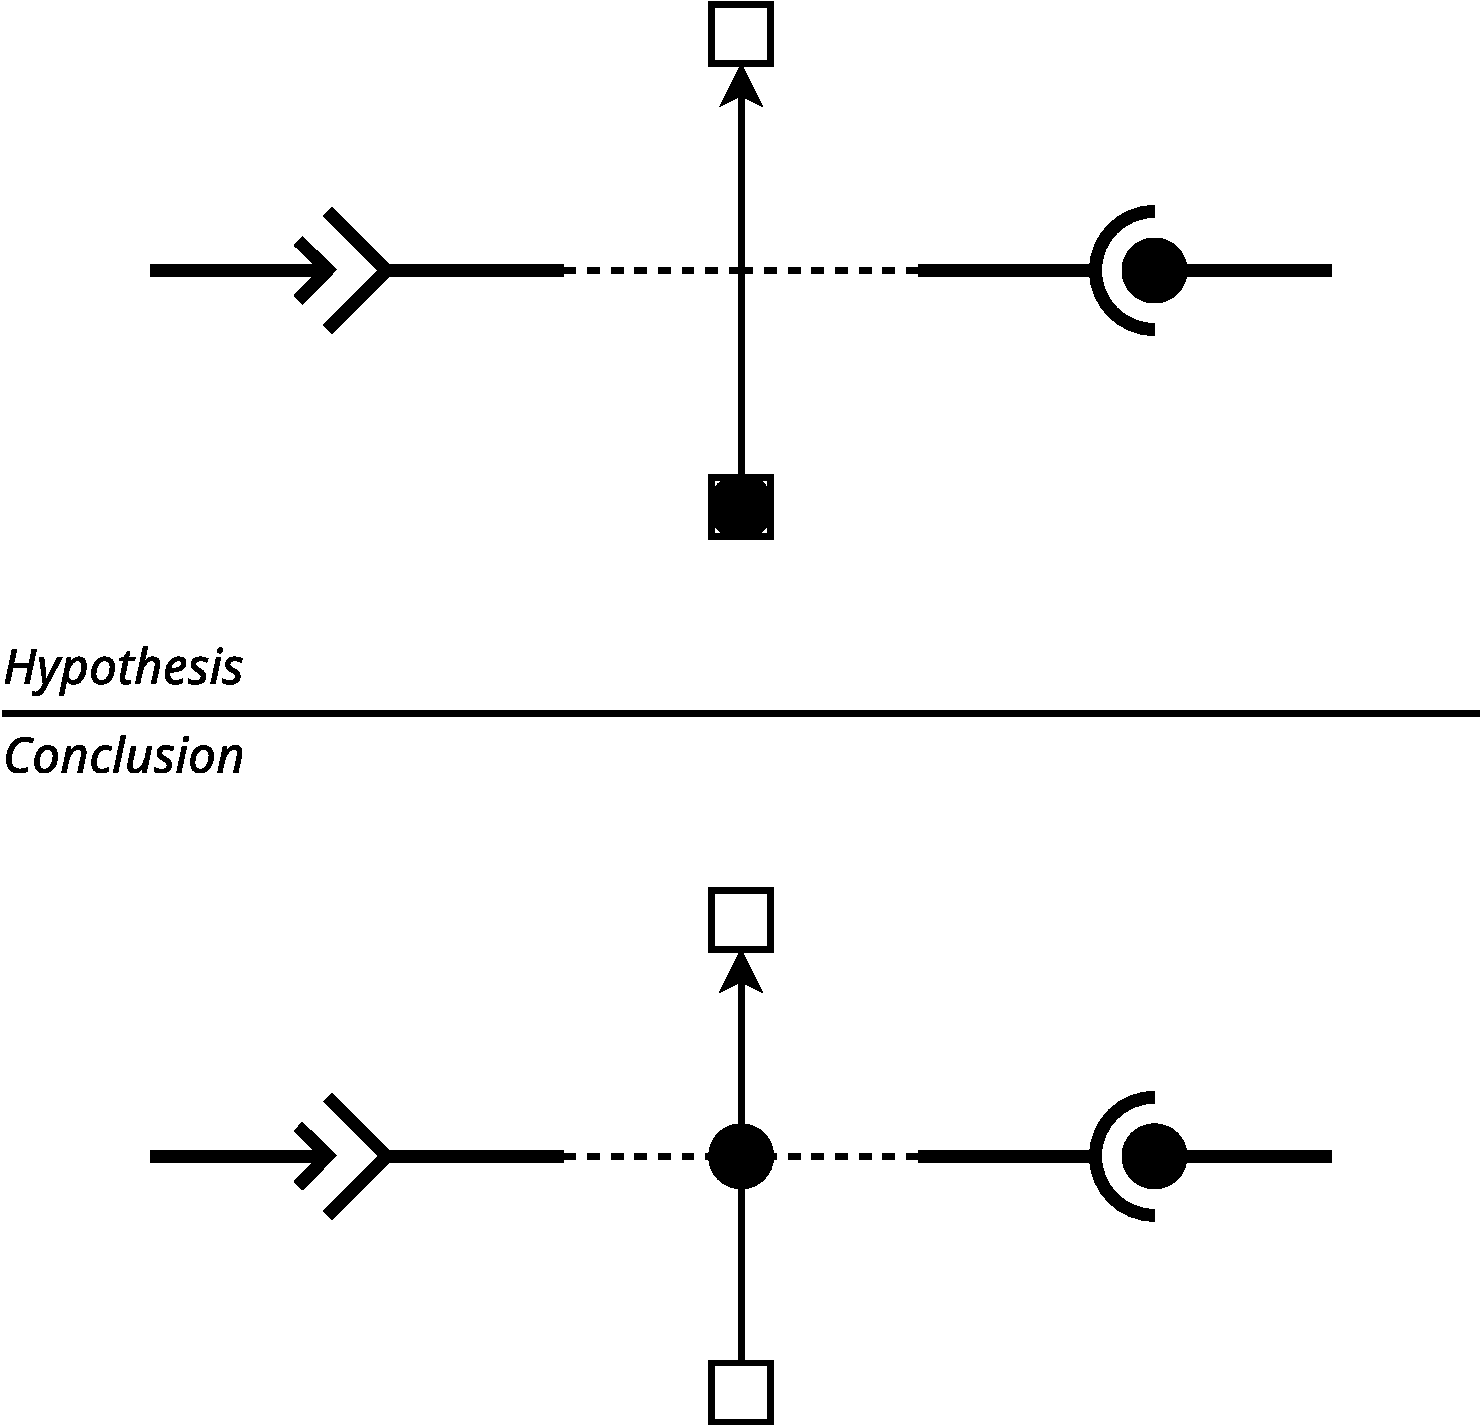
\includegraphics[width=0.55\columnwidth]{./images/firing.pdf}
\end{center}
\caption{Illustration of the rule of Equation~(\ref{eq:r1}) to fire transitions.}
\label{fig:r1}
\end{figure}

}

\paragraph{Ending transition}{

The second rule of \mad is formally defined by
Equation~(\ref{eq:r2}). To end a transition $\theta$, a token has to
be present on the transition and the action performed by the
transition must be terminated. When ending a transition, the token
is moved from this transition to its destination dock. Note that the ports bound
to the transition cannot be disconnected before applying this rule. Moreover, if
the place to which the destination dock is attached is bound to
data-provide ports, their values are replaced by those computed by the action.
For this reason, the rule uses the function
$val_{A,D_p}$. Figure~\ref{fig:r2} illustrates this rule.
%\MC{Expliquer pourquoi les ports ne peuvent pas etre deconnectes ?}

\begin{figure}[t]
\begin{center}
  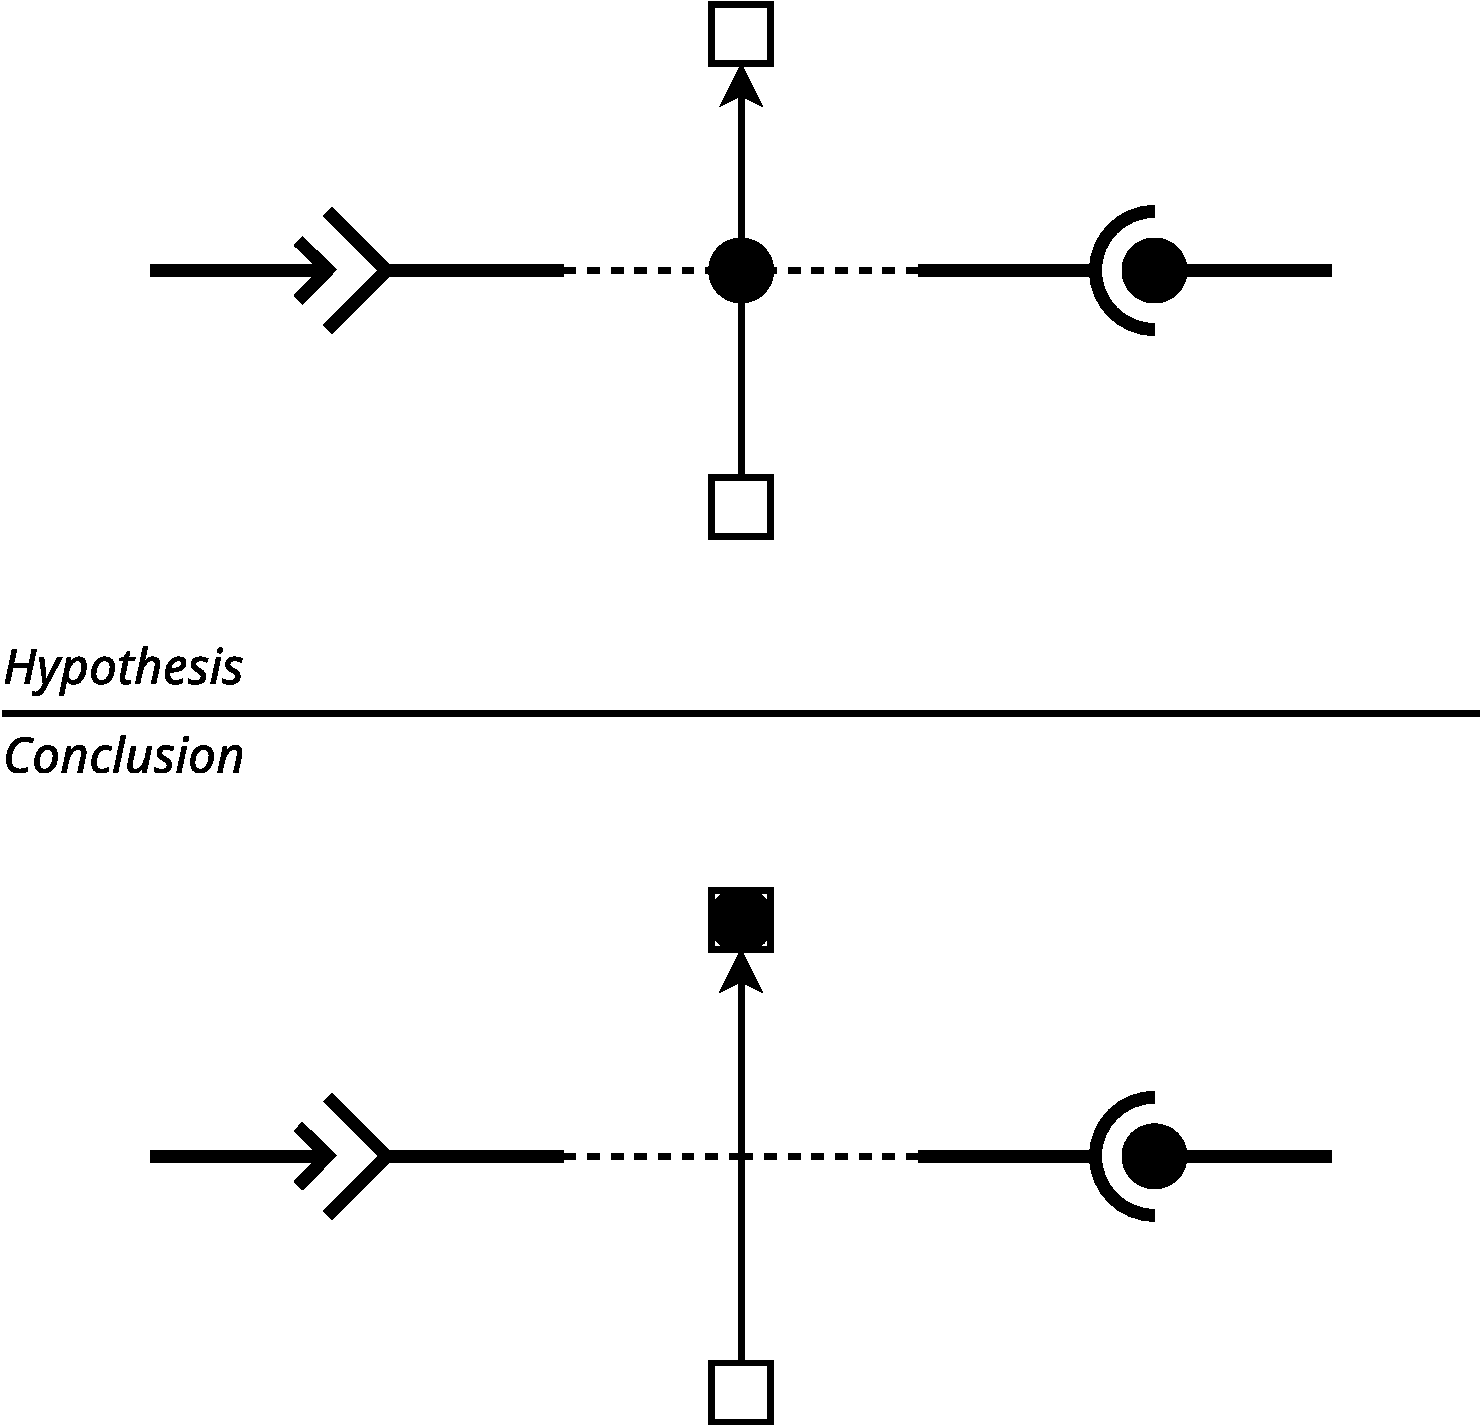
\includegraphics[width=0.55\columnwidth]{./images/ending_transition.pdf}
\end{center}
\caption{Illustration of the rule of Equation~(\ref{eq:r2}) to end transitions.}
\label{fig:r2}
\end{figure}
  
}

\paragraph{Input docks to place}{

The third rule of \mad is formally defined by
Equation~(\ref{eq:r3}). To move tokens from input docks of a place to
this place, all input docks must hold a token. The conclusion is to remove
all the tokens within the docks and to add one token inside the
place as illustrated in Figure~\ref{fig:r3}.

\begin{figure}[t]

\begin{minipage}[h]{0.45\columnwidth}%
  \centering
  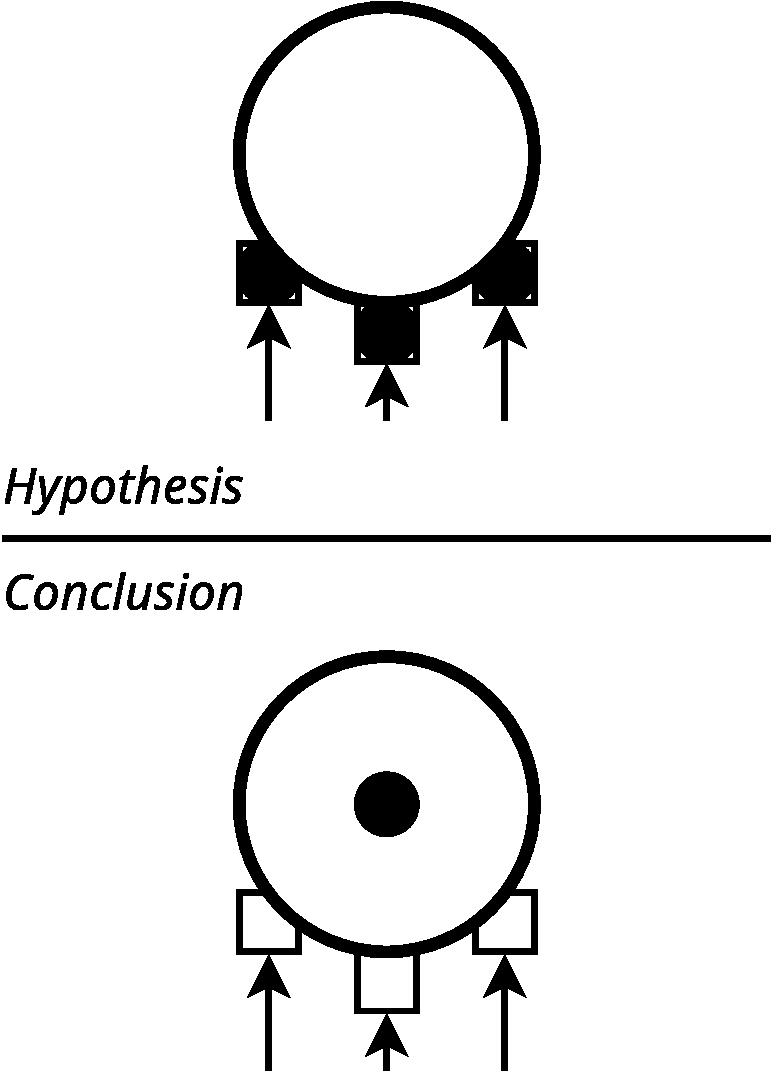
\includegraphics[width=0.65\columnwidth]{./images/inputdocks_to_place.pdf}
  \captionof{figure}{\label{fig:r3}Illustration of the rule of Equation~(\ref{eq:r3}) to move tokens from input docks to a place.}
\end{minipage}
\hfill
\begin{minipage}[h]{0.45\columnwidth}%
  \centering
  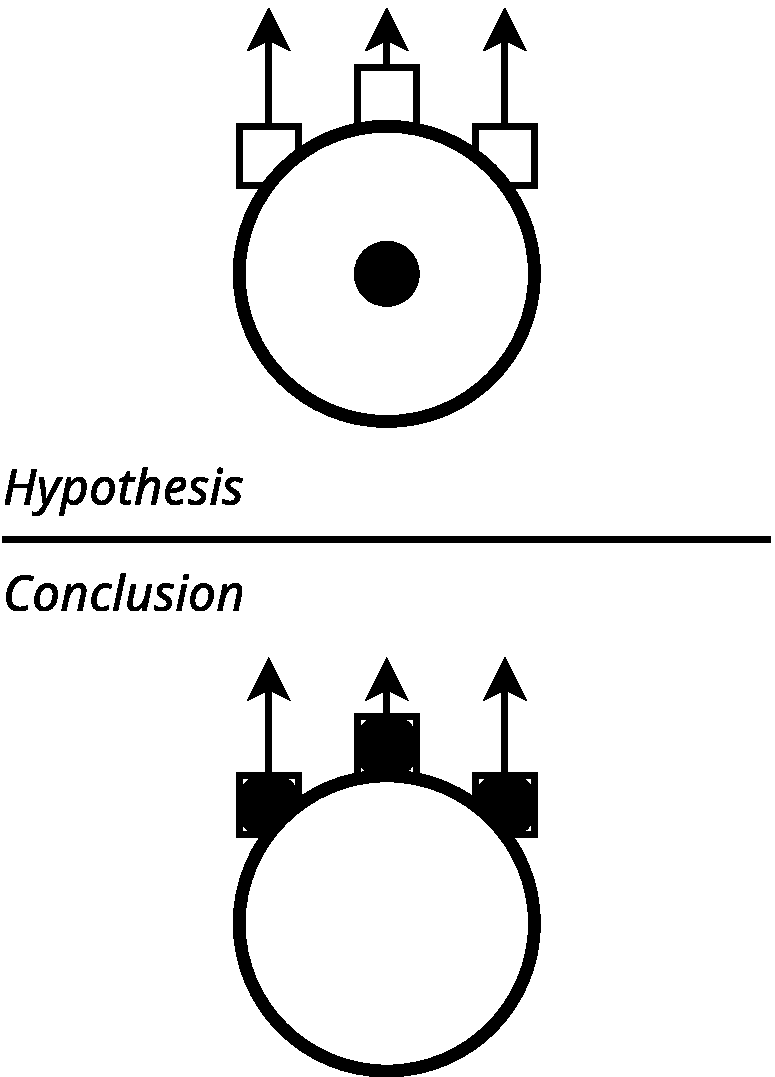
\includegraphics[width=0.65\columnwidth]{./images/place_to_outputdocks.pdf}
  \captionof{figure}{\label{fig:r4}Illustration of the rule of Equation~(\ref{eq:r4}) to move tokens from place to output docks.}
\end{minipage}
\end{figure}

\paragraph{Place to output docks}{

The fourth rule of \mad is formally defined by
Equation~(\ref{eq:r4}). To move a token from a place to its output
docks, a token needs to be present onto the place. Also, if the place
is part of a group which is itself bound to a used provide port,
applying the rule must not make the last token of the group leave,
otherwise this provide port becomes inactive. A provide port is said
to be used if it is connected to a use port bound to a transition
holding a token.  If these conditions are met, the token can be
removed from the place, and a token is added onto each output dock
attached to this place. This rule is illustrated in
Figure~\ref{fig:r4} in a simplified manner.

}

\paragraph{Enabling use-provide connections}{

The fifth rule of \mad is formally defined by
Equation~(\ref{eq:r5}). To enable a connection between use and provide
ports, at least one token has to be present in each group of places
bound to the provide port. A token is considered present in a group if
it is placed on one of the places, or on a transition between docks,
one of these docks being attached to one place of the group. The
conclusion of the rule is the enabling of the connection as depicted
in Figure~\ref{fig:r5}.

\begin{figure}[t]
  \begin{center}
    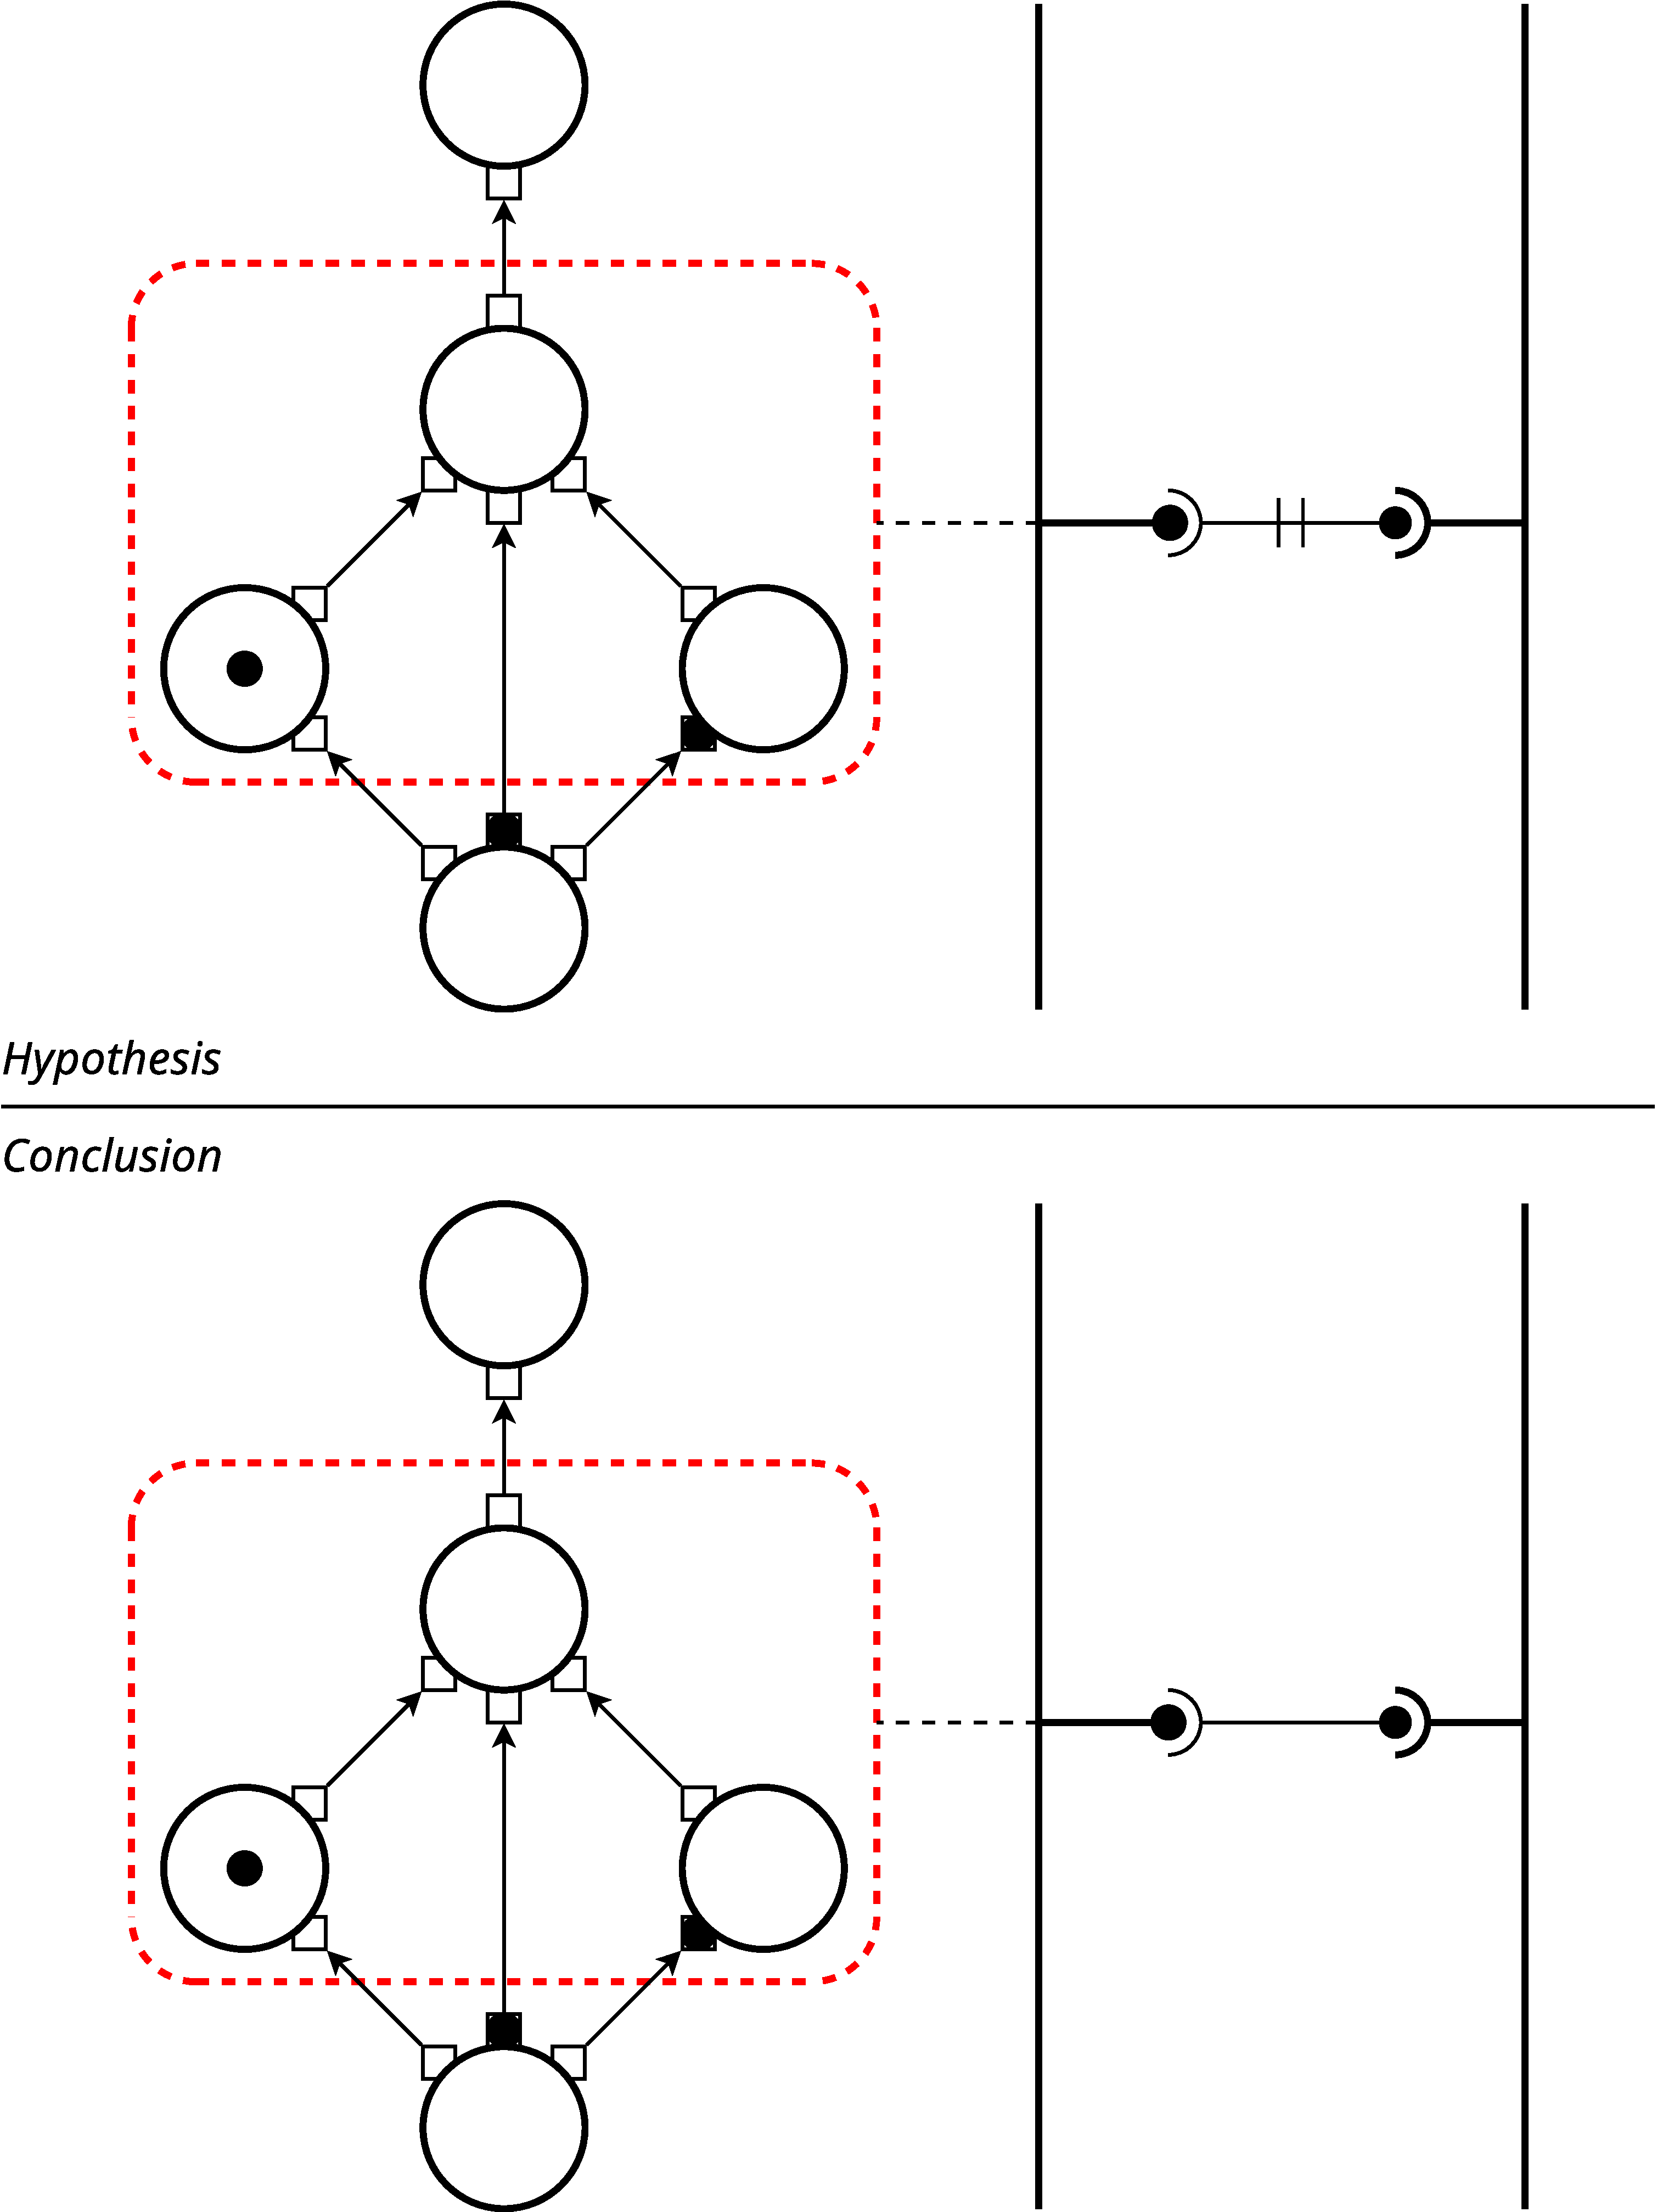
\includegraphics[width=0.7\columnwidth]{./images/link_service.pdf}

    \caption{Illustration of the rule of Equation~(\ref{eq:r5}) to enable a
    connection between use and provide ports of an assembly.}

    \label{fig:r5}
  \end{center}
\end{figure}
  
}

\paragraph{Disabling use-provide connections}{

The sixth rule of \mad is formally defined by
Equation~(\ref{eq:r6}). Note that this rule has maximum priority and
must be executed first if applicable. To disable a connection between
use and provide ports, there must not be any token in any group of
places bound to the provide port. The conclusion of the rule is to disable
the connection as depicted in Figure~\ref{fig:r6}.

\begin{figure}[t]
\begin{center}
  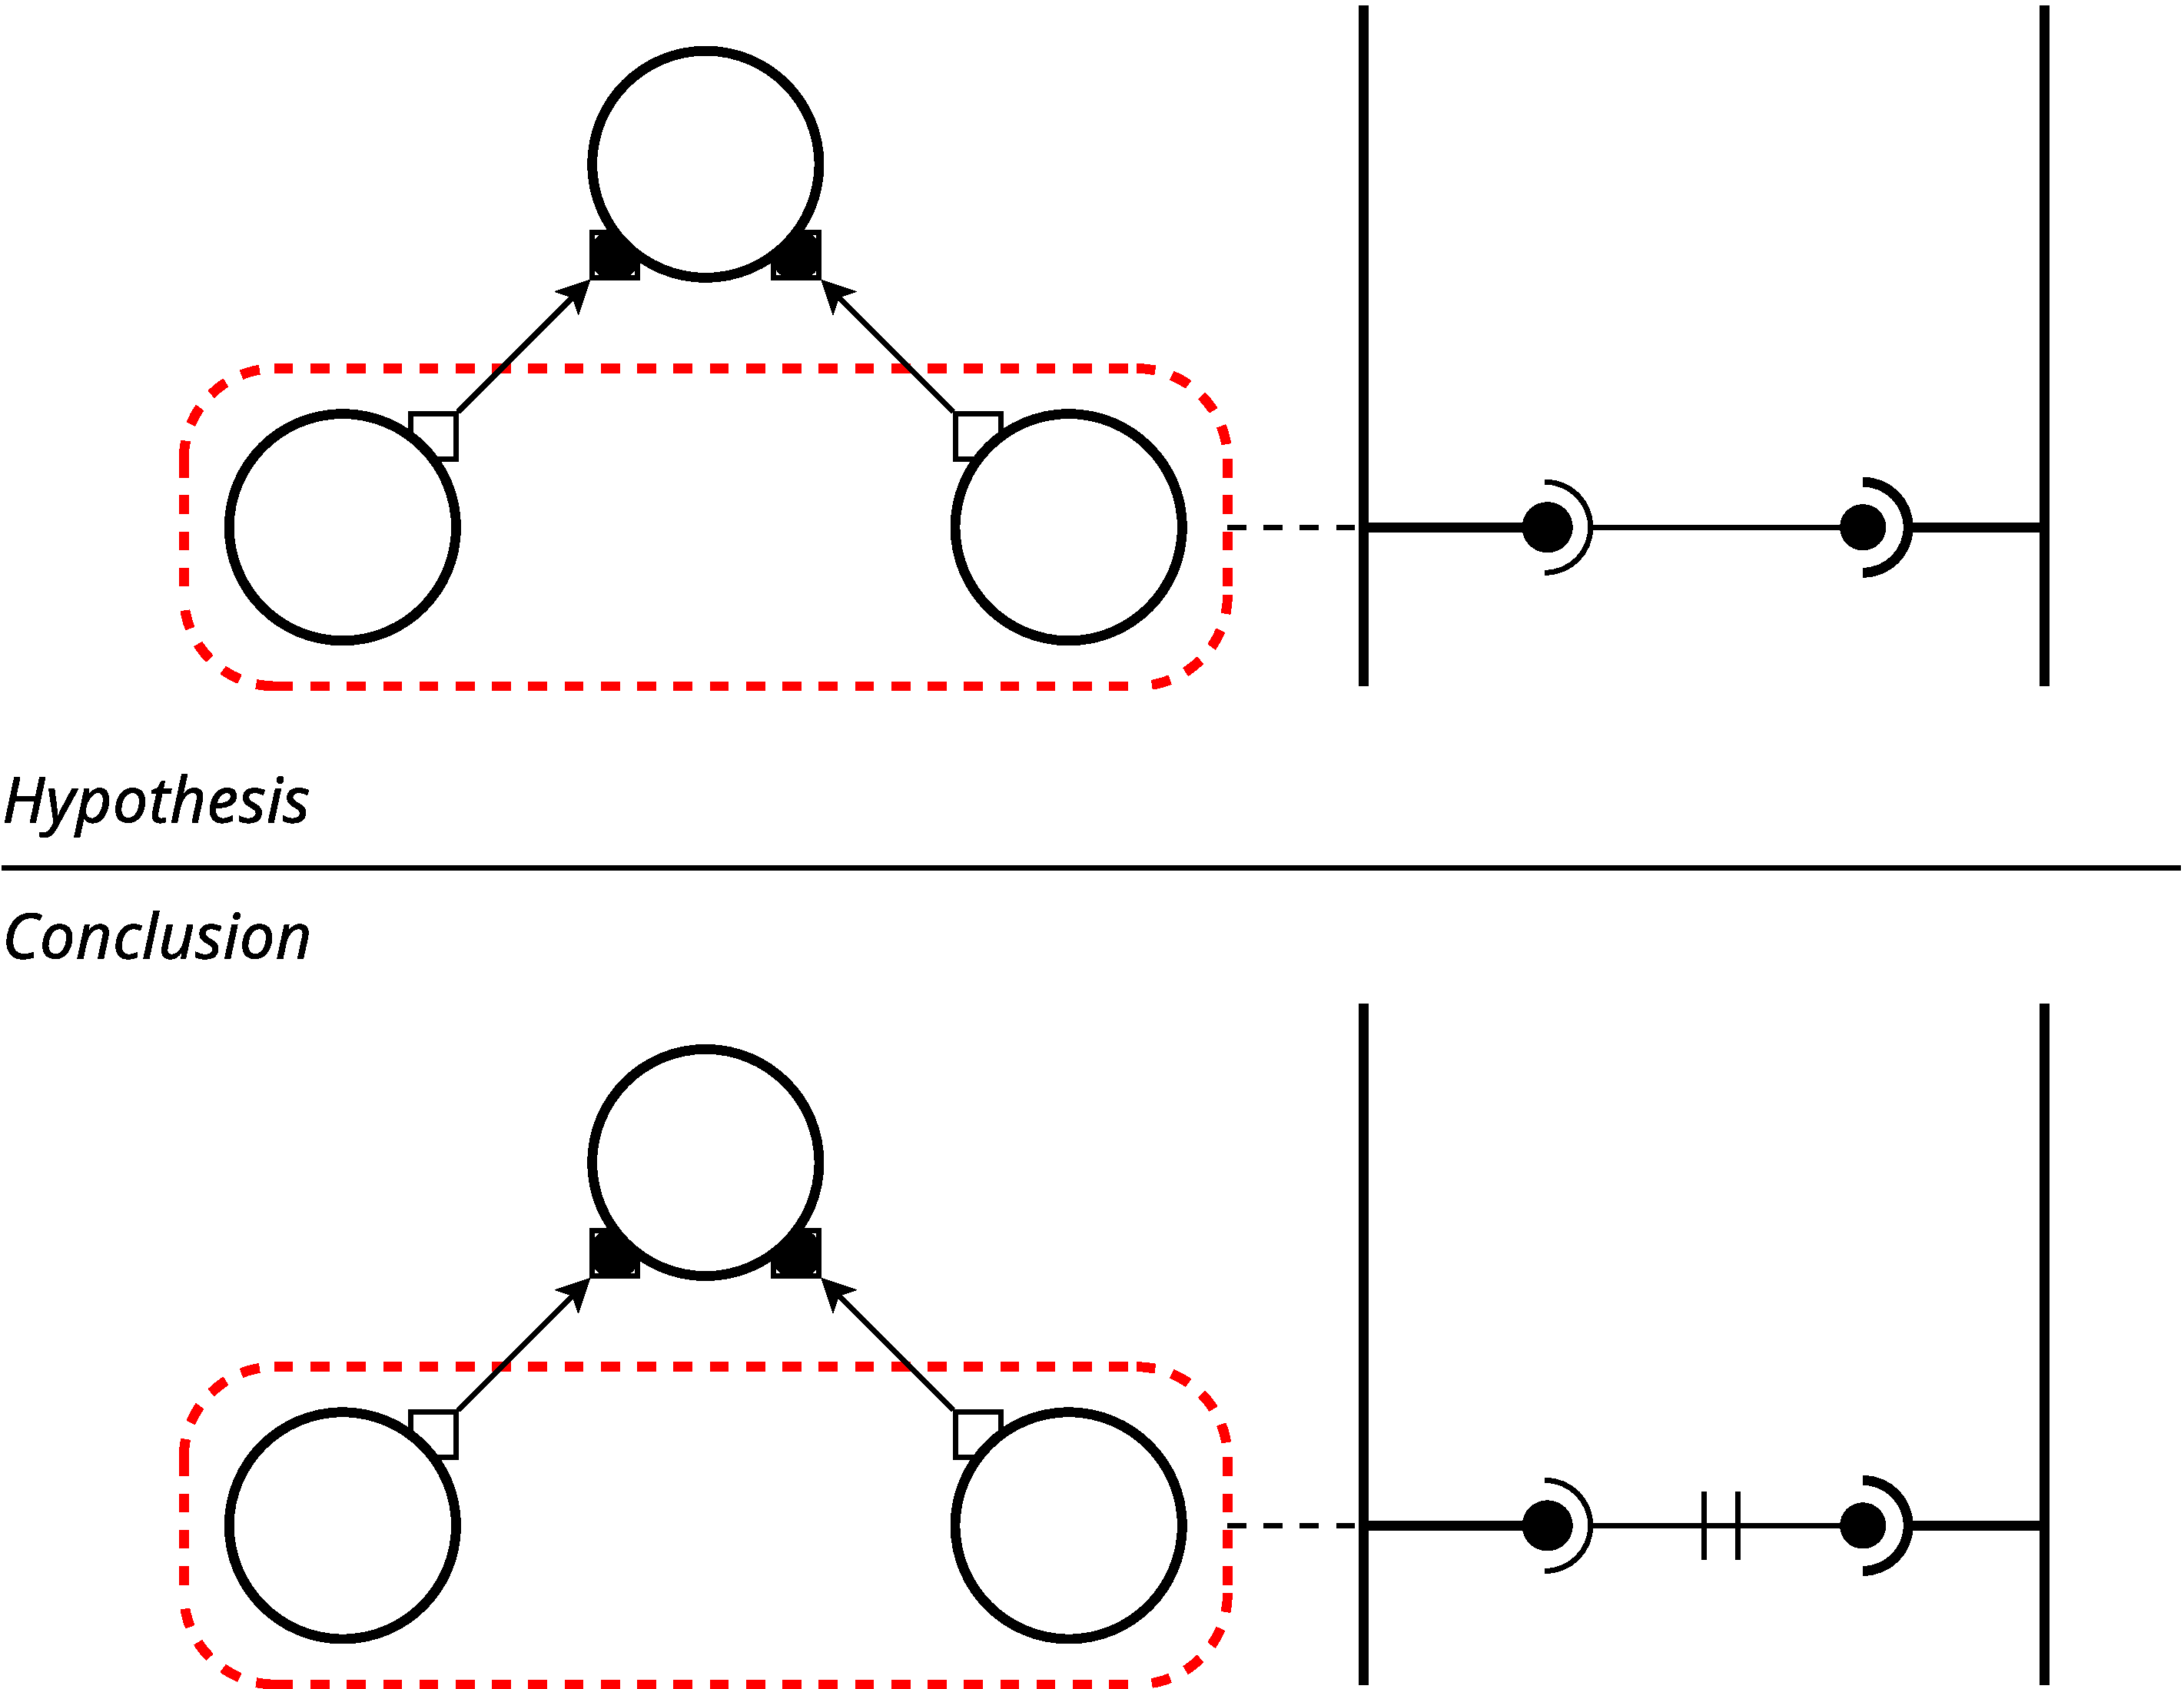
\includegraphics[width=0.7\columnwidth]{./images/break_service.pdf}
\end{center}
\caption{Illustration of the rule of Equation~(\ref{eq:r6}) to disable a connection between use and provide ports of an assembly.}
\label{fig:r6}
\end{figure}

}

\paragraph{Enabling data-use-provide connections}{

Finally, the seventh rule of \mad is formally defined by
Equation~(\ref{eq:r7}). To enable a connection between data-use and
data-provide ports, a value has to be associated to the data-provide
port. The conclusion of the rule is the activation of the connection as
depicted in Figure~\ref{fig:r7}. One can note that the position of
tokens is not a hypothesis in this rule. Actually, we consider in
the formal model that once a value has been attached to a data-provide
port, by applying the rule that ends a transition
(Equation~(\ref{eq:r2})), the connection of this port can be enabled
and will never be disabled. In pratice though, a disabling rule for
data ports could be usefull to not consume extra resources.
  
\begin{figure}[t]
\begin{center}
  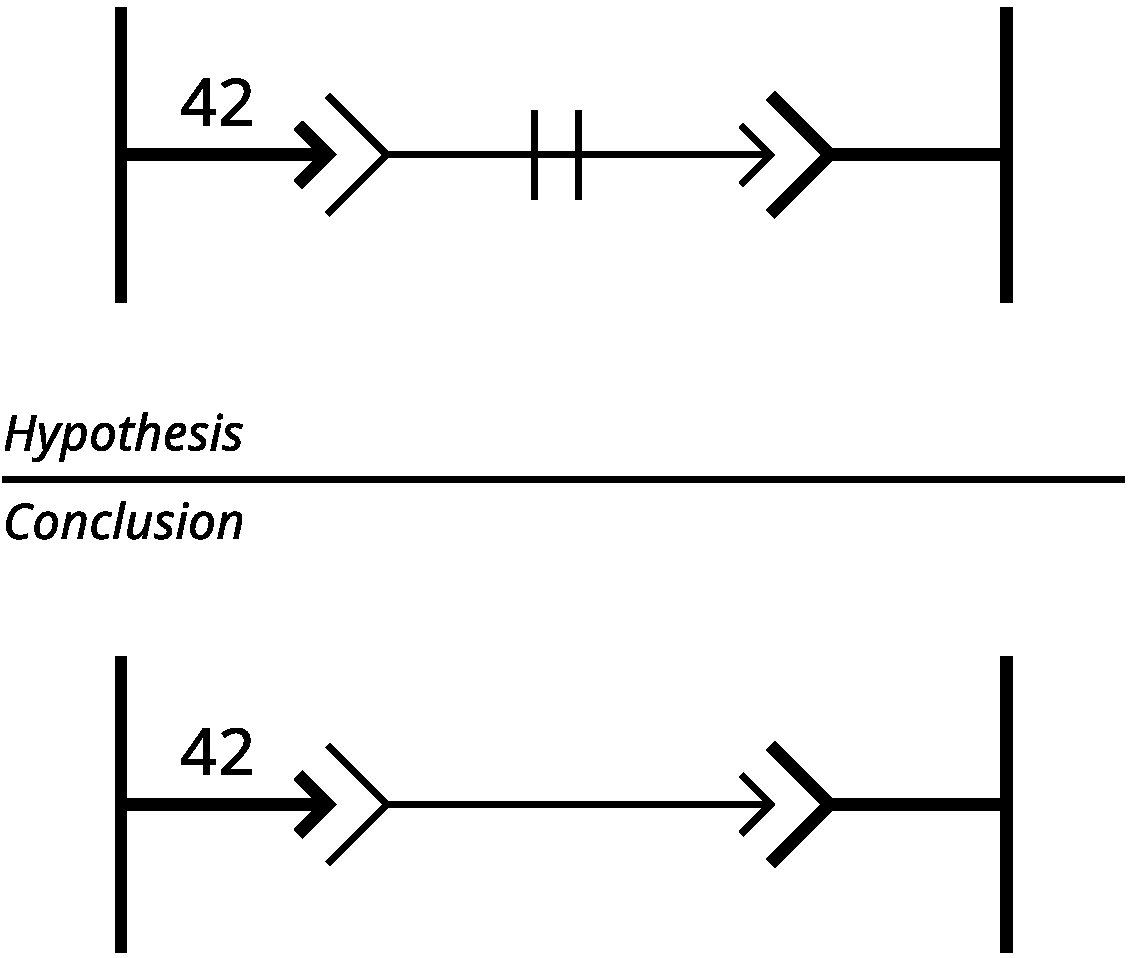
\includegraphics[width=0.4\columnwidth]{./images/link_data.pdf}
\end{center}
\caption{Illustration of the rule of Equation~(\ref{eq:r7}) to enable a connection between data-use and data-provide ports of an assembly.}
\label{fig:r7}
\end{figure}

}

%------------
\begin{figure*}[tp]
%
\begin{equation}
\cfrac{\theta =\left(s,d\right) \in \Theta^*,s \in \Delta_o^*,d \in \Delta_i^*\qquad mk\left(s\right)\qquad\forall p \in P_{u}\cup D_{u},\left(p,\theta\right)\in B_{P_{u}}^{*}\cup B_{D_{U}}^{*}\,:\,\text{is\_ready}(p)}{\left\langle mk,ebl,val\right\rangle \rightarrow\left\langle mk\left[s\coloneqq\text{false}\right]\left[\theta\coloneqq\text{true}\right],ebl,val\right\rangle }
\label{eq:r1}
\end{equation}
%
\begin{equation*}
  \text{where: }\text{is\_ready}(p) = \exists\left(a,b\right)\in L_{S}\cup L_{D},\,a=p\land ebl\left(a,b\right).
\end{equation*}
%
\begin{equation}
\cfrac{\theta=\left(s,d\right) \in \Theta^*\qquad mk\left(\theta\right)\qquad end\left(action\left(\theta\right)\right)}{\left\langle mk,ebl,val\right\rangle \rightarrow\left\langle mk\left[\theta\coloneqq\text{false}\right]\left[d\coloneqq\text{true}\right],ebl,val\left[\forall p\in D_P^*,\text{dest}(p)\,:\, p\coloneqq val_{A,D_p}(action(\theta),p)\right]\right\rangle}
\label{eq:r2}
\end{equation}
%
\begin{equation*}
  \text{where: }\text{dest}(p) = \left(p,g\right)\in B_{D_{p}}^*,place(d)\in g
\end{equation*}
%
\begin{equation}
\cfrac{\pi\in\Pi^*\qquad D_i=dock_i(\pi)\qquad\forall\delta\in D_i\,mk\left(\delta\right)}{\left\langle mk,ebl,val\right\rangle \rightarrow\left\langle mk\left[\forall\delta\in D_i\,:\,\delta\coloneqq\text{false}\right]\left[\pi\coloneqq\text{true}\right],ebl,val\right\rangle }
\label{eq:r3}
\end{equation}
%
\begin{equation}
\cfrac{\pi\in\Pi^{*}\qquad D_o=dock_o(\pi)\qquad mk\left(\pi\right)\qquad \forall g\in G,\pi\in g:\,\text{can\_leave}\left(\pi,D_o,g\right)}{\left\langle mk,ebl,val\right\rangle \rightarrow\left\langle mk\left[\forall\delta\in D_o\,:\,\delta\coloneqq\text{true}\right]\left[\pi\coloneqq\text{false}\right],ebl,val\right\rangle }
\label{eq:r4}
\end{equation}
%
\begin{align*}
\text{where: }\text{can\_leave}\left(\pi,D_o,g\right) = & \left(\exists p,(p,g)\in B_{P_p}:\,\text{is\_used}(p)\right)\implies \lnot \text{last\_token\_leaves} \left(\pi,D_o,g\right) \\
\text{is\_used}\left(p\right) = & \exists u\in P_{u}^{*},\theta\in\Theta^{*}:~\left(p,u\right)\in L_{P}\land \left(u,\theta\right)\in B_{P_u}^{*}\land mk\left(\theta\right) \\
\text{last\_token\_leaves}\left(\pi,D_o,g\right) = & \left(\text{is\_group\_enabled}\left(g,mk\right)\land\lnot \text{is\_group\_enabled} \left(g,mk\left[\pi\coloneqq \text{false}\right]\left[\forall d\in D_o \,:\,d\coloneqq \text{true}\right]\right)\right) \\
\text{is\_group\_enabled}\left(g,mk\right) = & \left(\exists\,\pi\in g:\,mk\left(\pi\right)\right)\\
 & \, \lor\left(\exists\,\delta\in\Delta_{o}^{*}\cup\Delta_{i}^{*}:\,mk\left(\delta\right)\land \left(\exists(s,d)\in\Theta^{*}:\,\left(\delta=s\lor \delta=d\right)\land \text{is\_in\_group}\left((s,d),g\right)\right)\right)\\
 & \, \lor\left(\exists\,\theta\in\Theta^{*}:\,mk\left(\theta\right)\land \text{is\_in\_group}\left(\theta,g\right)\right) \\
\text{is\_in\_group}\left((s,d),g\right) = & place\left(s\right)\in g\land place\left(d\right)\in g
\end{align*}
%
\begin{equation}
\cfrac{l = (u,p)\in L_{S}\qquad\lnot ebl\left(l\right)\qquad\forall g \in G,\left(p,g\right)\in B_{P_{p}}\,:\,\text{is\_group\_enabled}\left(g,mk\right)}{\left\langle mk,ebl,val\right\rangle \rightarrow\left\langle mk,ebl\left[l\coloneqq\text{true}\right],val\right\rangle }
\label{eq:r5}
\end{equation}
%
\begin{equation}
\cfrac{l=(u,p)\in L_{S}\qquad ebl\left(l\right)\qquad\exists g \in G,\left(p,g\right)\in B_{P_{p}}\,:\,\lnot\text{is\_group\_enabled}\left(g,mk\right)}{\left\langle mk,ebl,val\right\rangle \rightarrow\left\langle mk,ebl\left[l\coloneqq\text{false}\right],val\right\rangle }
\label{eq:r6}
\end{equation}
%
\begin{equation}
\cfrac{l=(u,p)\in L_{D}\qquad\lnot ebl\left(l\right)\qquad val\left(p\right)\neq\text{null}}{\left\langle mk,ebl,val\right\rangle \rightarrow\left\langle mk,ebl\left[l\coloneqq\text{true}\right],val\right\rangle }
\label{eq:r7}
\end{equation}
%
\caption{The seven operational semantics rules of \mad.}
\label{fig:rules}
\end{figure*}
%------------

%--------------------------
%\subsection{Consistency rule}
%--------------------------
\textbf{Consistency.}

In \mad, the maximum number of tokens that can be used is the number
of possible parallel branches. A token can only be created during a
branching (rule \emph{place to output docks}), where one token is
created for each output dock of the place. For this reason, cycles are
forbidden in \mad, otherwise an infinity of tokens could be created
which does not make sense within a deployment. We plan in future work
on reconfiguration to allow cycles in very specific settings to keep
control on the tokens and their creation.

\HC[All]{Maybe the performance model in this section too if short
  enough}